

\tikzset{every picture/.style={line width=0.75pt}} %set default line width to 0.75pt        
\begin{center}
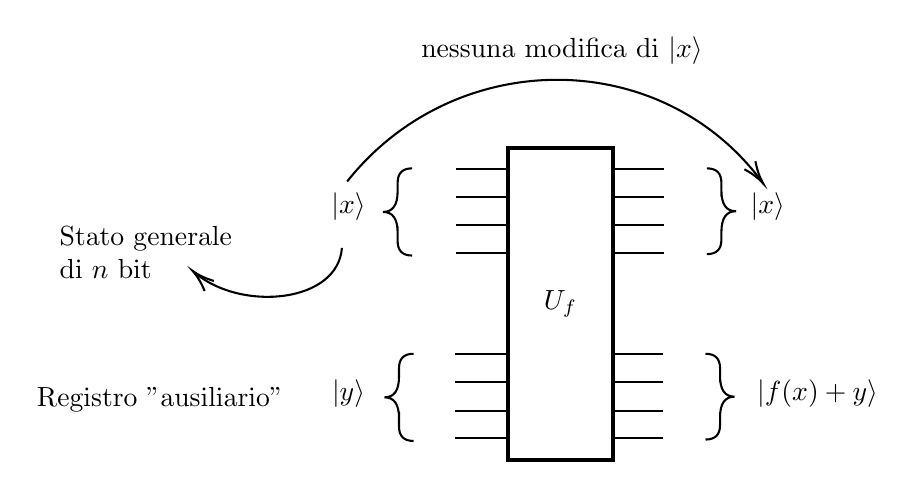
\begin{tikzpicture}[x=0.75pt,y=0.75pt,yscale=-1,xscale=1]
%uncomment if require: \path (0,300); %set diagram left start at 0, and has height of 300

%Straight Lines [id:da8018762189626685] 
\draw    (240.67,130.33) -- (265.46,130.33) ;


%Straight Lines [id:da9959980995216082] 
\draw    (240.67,117.11) -- (265.46,117.11) ;


%Straight Lines [id:da7944941960941587] 
\draw    (240.67,103.44) -- (265.46,103.44) ;


%Straight Lines [id:da634487408707328] 
\draw    (240.67,90) -- (265.46,90) ;


%Shape: Rectangle [id:dp021998310168785284] 
\draw  [line width=1.5]  (265.46,80) -- (316.2,80) -- (316.2,230.33) -- (265.46,230.33) -- cycle ;
%Straight Lines [id:da030079298074298544] 
\draw    (240,219.67) -- (264.79,219.67) ;


%Straight Lines [id:da2512264773728652] 
\draw    (240,206.45) -- (264.79,206.45) ;


%Straight Lines [id:da4910617169628535] 
\draw    (240,192.78) -- (264.79,192.78) ;


%Straight Lines [id:da5560947433565258] 
\draw    (240,179.33) -- (264.79,179.33) ;


%Straight Lines [id:da5981123718501302] 
\draw    (316.65,130.33) -- (340.67,130.33) ;


%Straight Lines [id:da7695634239792029] 
\draw    (316.65,117.11) -- (340.67,117.11) ;


%Straight Lines [id:da223585002874922] 
\draw    (316.65,103.44) -- (340.67,103.44) ;


%Straight Lines [id:da8717396364570034] 
\draw    (316.65,90) -- (340.67,90) ;


%Straight Lines [id:da07009581136174425] 
\draw    (316,219.67) -- (340.02,219.67) ;


%Straight Lines [id:da425350873363203] 
\draw    (316,206.45) -- (340.02,206.45) ;


%Straight Lines [id:da6575106053976216] 
\draw    (316,192.78) -- (340.02,192.78) ;


%Straight Lines [id:da13811669103293145] 
\draw    (316,179.33) -- (340.02,179.33) ;


%Shape: Brace [id:dp19177418456346462] 
\draw   (219.33,89.67) .. controls (214.66,89.67) and (212.33,92) .. (212.33,96.67) -- (212.33,100.67) .. controls (212.33,107.34) and (210,110.67) .. (205.33,110.67) .. controls (210,110.67) and (212.33,114) .. (212.33,120.67)(212.33,117.67) -- (212.33,124.67) .. controls (212.33,129.34) and (214.66,131.67) .. (219.33,131.67) ;
%Shape: Brace [id:dp7848695493053537] 
\draw   (220,179) .. controls (215.33,179) and (213,181.33) .. (213,186) -- (213,190) .. controls (213,196.67) and (210.67,200) .. (206,200) .. controls (210.67,200) and (213,203.33) .. (213,210)(213,207) -- (213,214) .. controls (213,218.67) and (215.33,221) .. (220,221) ;
%Shape: Brace [id:dp6879081564155314] 
\draw   (361.33,131) .. controls (366,131) and (368.33,128.67) .. (368.33,124) -- (368.33,120.33) .. controls (368.33,113.66) and (370.66,110.33) .. (375.33,110.33) .. controls (370.66,110.33) and (368.33,107) .. (368.33,100.33)(368.33,103.33) -- (368.33,96.67) .. controls (368.33,92) and (366,89.67) .. (361.33,89.67) ;
%Shape: Brace [id:dp004338255968296956] 
\draw   (360.67,220.33) .. controls (365.34,220.33) and (367.67,218) .. (367.67,213.33) -- (367.67,209.67) .. controls (367.67,203) and (370,199.67) .. (374.67,199.67) .. controls (370,199.67) and (367.67,196.34) .. (367.67,189.67)(367.67,192.67) -- (367.67,186) .. controls (367.67,181.33) and (365.34,179) .. (360.67,179) ;
%Curve Lines [id:da07561091183948077] 
\draw    (185.5,128) .. controls (183.54,154.46) and (137.4,158.83) .. (114.85,140.17) ;
\draw [shift={(113.5,139)}, rotate = 402.27] [color={rgb, 255:red, 0; green, 0; blue, 0 }  ][line width=0.75]    (10.93,-3.29) .. controls (6.95,-1.4) and (3.31,-0.3) .. (0,0) .. controls (3.31,0.3) and (6.95,1.4) .. (10.93,3.29)   ;

%Curve Lines [id:da4879607381242139] 
\draw    (188,96) .. controls (239.74,30.83) and (339,30.5) .. (387.77,96.01) ;
\draw [shift={(388.5,97)}, rotate = 233.9] [color={rgb, 255:red, 0; green, 0; blue, 0 }  ][line width=0.75]    (10.93,-3.29) .. controls (6.95,-1.4) and (3.31,-0.3) .. (0,0) .. controls (3.31,0.3) and (6.95,1.4) .. (10.93,3.29)   ;


% Text Node
\draw (290.83,155.17) node   {$U_{f}$};
% Text Node
\draw (188.67,108) node   {$|x\rangle $};
% Text Node
\draw (188.67,198) node   {$|y\rangle $};
% Text Node
\draw (390.67,108) node   {$|x\rangle $};
% Text Node
\draw (414.67,198) node   {$|f( x) +y\rangle $};
% Text Node
\draw (98,201) node  [align=left] {Registro "ausiliario"};
% Text Node
\draw (91,130) node  [align=left] {Stato generale\\di $\displaystyle n$ bit};
% Text Node
\draw (291.5,33) node  [align=left] {nessuna modifica di $\displaystyle |x\rangle $};


\end{tikzpicture}
\end{center}